%% V1.0
%% by Tan Kai Xiong, legendarykx.kaixiong1@gmail.com
%% This is a template for Udacity projects using IEEEtran.cls

%% Be Udacious!

\documentclass[10pt,journal,compsoc]{IEEEtran}

\usepackage[pdftex]{graphicx}    
\hyphenation{op-tical net-works semi-conduc-tor}


\begin{document}

\title{Where Am I?}

\author{Tan Kai Xiong}

\markboth{Localization project, Robotic Nanodegree, Udacity}%
{}
\IEEEtitleabstractindextext{%

\begin{abstract}
The goal of the project is to make use of ROS (Robotics Operating System) packages to accurately localize a mobile robot inside a provide map in the Gazebo and RViz simulation environments. A custom differential wheel mobile robot model will be created in a Gazebo world. ROS navigation stack is applied in this project, packages such as AMCL (Adaptive Monte Carlos Localization), Map Server and Move Base. Depend on compute platform and sensor accuracy, performance tuning is required to achieve the best localization results. 
\end{abstract}

% Note that keywords are not normally used for peerreview papers.
\begin{IEEEkeywords}
Robot, IEEEtran, Udacity, \LaTeX, AMCL, Localization.
\end{IEEEkeywords}}


\maketitle
\IEEEdisplaynontitleabstractindextext
\IEEEpeerreviewmaketitle
\section{Introduction}
\label{sec:introduction}

\IEEEPARstart{T}{he} objective of this project is to use ROS packages to localize a mobile robot inside a provided map in the Gazebo and RViz simulation environments. This article will present an overview of a navigation stack in ROS.

\begin{itemize}
\item Create a custom ROS package
\item Write a custom robot model in a Gazebo world
\item Write launch script to bring up the custom robot in the Gazebo world
\item Write launch script to launch AMCL and Move\_Base packages
\item Tune the AMCL parameter to achieve the best possible localization results
\end {itemize}

\section{Robot Model}
A custom differential wheel mobile robot is built in URDF file.  For this type of wheel drive,
it requires two independent motor driven wheels to enable this type of driver to work. It can have either one or two caster wheels to support the robot. It consists of a hokuyo laser scanner, camera and differential wheel sensor.

\begin{figure}[thpb]
      \centering
      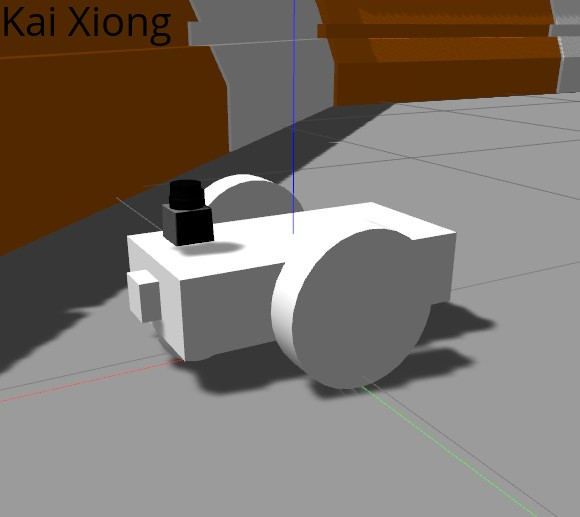
\includegraphics[scale=0.25]{Robot.jpg}
      \caption{Robot Model.}
      \label{fig:robot1}
\end{figure}

\section{Localization}
Localization is the basic function of a mobile robot. Before the robot can execute any movement, it need to determine its own position with respect to the map. With the ability of localization, the robot can navigate from point A to B. Mobile robot also must be able to avoid dangerous situations such as collisions and unsafe environment.

\subsection{EKF vs MCL}
The main two types of localization methods are “Extended Kalman Filter” and “Monte Carlo Localization”. MCL is a type of particle filter algorithm. Compare EFK with MCL, MCL is more robust and it capable of global localization.

\begin{table}[thpb]
\begin{tabular}{|l|l|l|}
\hline
                             & \textbf{EKF}        & \textbf{MCL}        \\ \hline
Observation                  & Landmarks           & Raw measurement     \\ \hline
Observation noise            & Gaussian            & Any                 \\ \hline
Posterior                    & Gaussian            & Particles           \\ \hline
Efficiency (Memory)          & Excellent           & Good                \\ \hline
Efficiency (Time)            & Excellent           & Good                \\ \hline
Ease of Implementation       & Good                & Excellent           \\ \hline
Resolution                   & Good                & Excellent           \\ \hline
Robustness                   & Bad                 & Excellent           \\ \hline
Memory \& Resolution Control & No                  & Yes                 \\ \hline
Global Localization          & No                  & Yes                 \\ \hline
State Space                  & Unimodel Continuous & Multimodel Discrete \\ \hline
\end{tabular}
\caption{EKF vs MCL comparison table.}
\label{tab:template1}
\end{table}

\section{AMCL}
AMCL (Adaptive Monte Carlo Localization) is a probabilistic localization package for 2D navigation. It implements the adaptive (or KLD-Sampling) Monte Carlo Localization approach which use a particle filter to track the pose of a robot with a known map. 

The AMCL pose output frequency is depended on the frequency rate of the laser scans. If the laser scan frequency is 10 Hz, the maximum output of the AMCL\_POSE will be 10 Hz. In order to make the particle converge quicker, by reducing the “update\_min\_d” and “update\_min\_a”.

AMCL would work well for the kidnapped robot problem as it can perform global localization.  It would require a known map. Global localization is being used if the robot do not know its initial position. There is a ROS service in AMCL which can trigger the global localization. The particles are dispersed randomly through the free space in the map. When the robot move, the particles are being updated and re-sampled. After a few iterations, the particle will converge.

\begin{table}[thpb]
\begin{tabular}{|l|l|}
\hline
\textbf{Parameters}  & \textbf{Value}   \\ \hline
odom\_frame\_id      & odom             \\ \hline
odom\_model\_type    & diff-corrected   \\ \hline
base\_frame\_id      & robot\_footprint \\ \hline
global\_frame\_id    & map              \\ \hline
min\_particles       & 10               \\ \hline
max\_particles       & 500              \\ \hline
transform\_tolerance & 0.1              \\ \hline
resample\_interval   & 1                \\ \hline
odom\_alpha1         & 0.05             \\ \hline
odom\_alpha2         & 0.05             \\ \hline
odom\_alpha3         & 0.05             \\ \hline
odom\_alpha4         & 0.05             \\ \hline
update\_min\_a       & 0.01             \\ \hline
update\_min\_d       & 0.01             \\ \hline
\end{tabular}
\caption{AMCL Parameters.}
\label{tab:template2}
\end{table}

\section{Move\_Base}
The move\_base package provides an implementation of an action (actionlib package) that, given a goal in the world, it will attempt to reach it with a mobile base. The move\_base node links together a global and local planner to accomplish its global navigation task. It supports any global planner adhering to the nav\_core::BaseGlobalPlanner interface specified in the nav\_core package and any local planner adhering to the nav\_core::BaseLocalPlanner interface specified in the nav\_core package.

\begin{table}[thpb]
\begin{tabular}{|l|l|}
\hline
\textbf{Parameters}   & \textbf{Value}       \\ \hline
base\_global\_planner & navfnNavfnROS        \\ \hline
base\_local\_planner  & TrajectoryPlannerROS \\ \hline
max\_vel\_x           & 0.5                  \\ \hline
min\_vel\_x`          & 0.1                  \\ \hline
xy\_goal\_tolerance   & 0.05                 \\ \hline
yaw\_goal\_tolerance  & 0.05                 \\ \hline
\end{tabular}
\caption{Move\_Base Parameters.}
\label{tab:template3}
\end{table}

\section{Map\_Server}
Map\_server provide the map\_server ROS Node, which offers map data as a ROS Service. It also provides the map\_saver command-line utility, which allows dynamically generated maps to be saved to file. It is used for loading static map.

\begin{figure}[thpb]
      \centering
      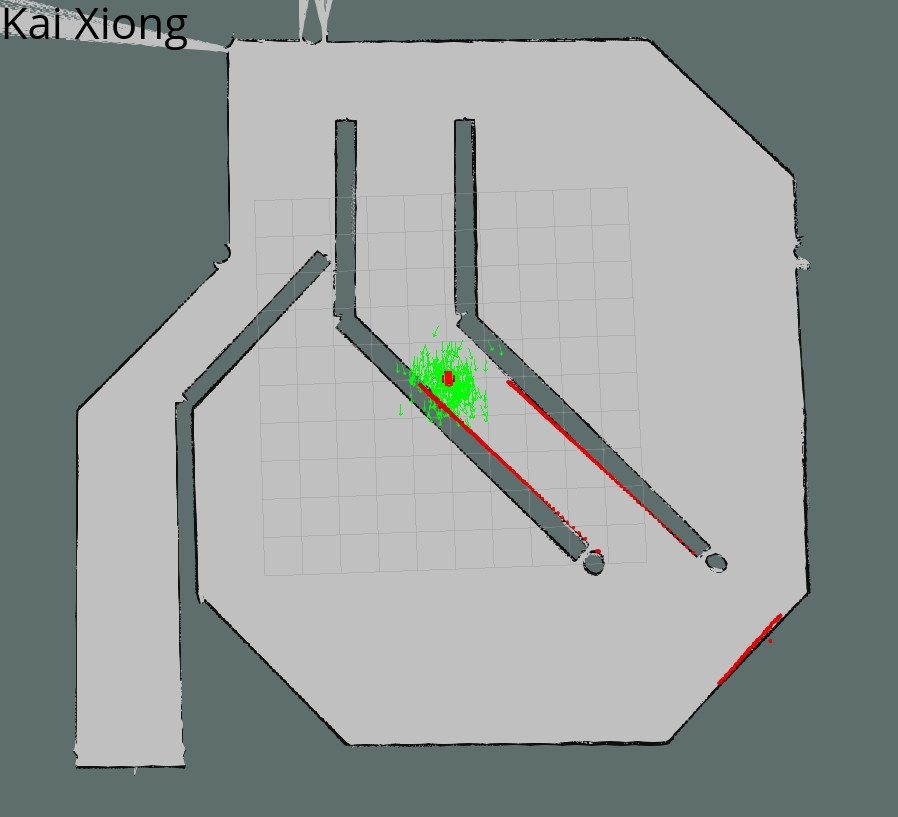
\includegraphics[scale=0.125]{map.jpg}
      \caption{Jackal Race 2D Grid-map.}
      \label{fig:robot2}
\end{figure}

\section{Localization Accuracy}
The AMCL output AMCL\_POSE message. The message type is geometry\_msgs/PoseWithCovarianceStamped. The localization accuracy is represented in the pose covariance. The 6x6 covariance matrix represent in x, y, z rotation about X axis, rotation about Z axis. The higher the value, it represent higher uncertainty.
Number of particles used in AMCL is depended on the map area and whether global localization is needed. Increase the number of particles will affect the processing time. If there is too few particle, the accuracy of the AMCL pose will decrease.
Reduce the update distance and angular will increase the update frequency, thus increase the processing time. It allow the particle to converge faster and the accuracy of the AMCL pose will increase.
The performance of AMCL also depend on the compute platform. If the compute platform CPU performance is slow, the user need to reduce the number of particle or increase the update distance and angular rate.

\section{Results}

\begin{figure}[thpb]
      \centering
      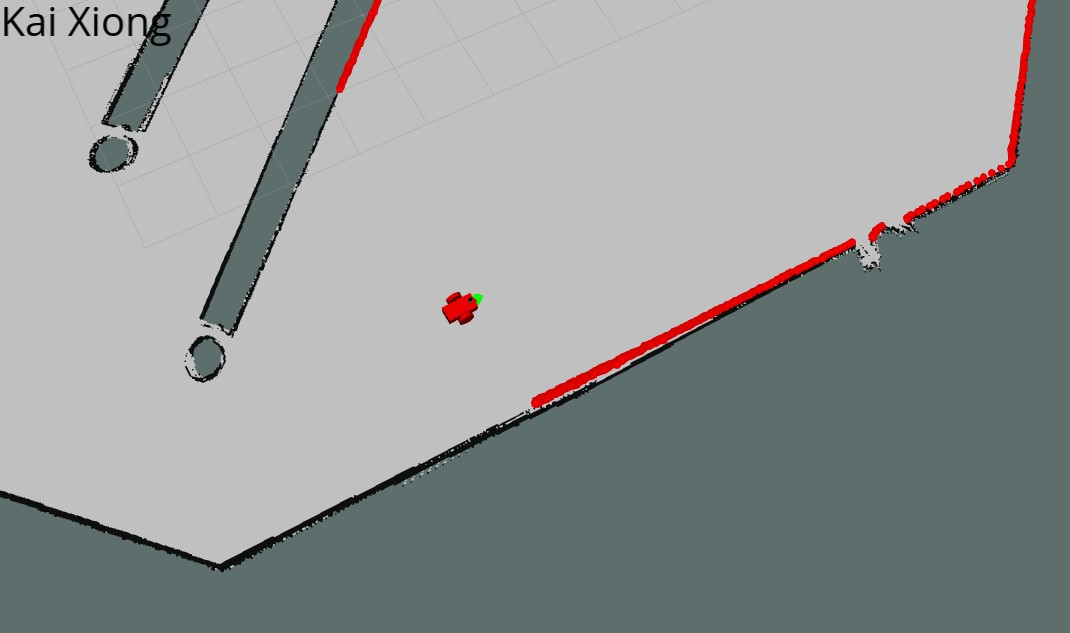
\includegraphics[width=\linewidth]{AMCL.jpg}
      \caption{Localized Map.}
      \label{fig:robot3}
\end{figure}

\begin{figure}[thpb]
      \centering
      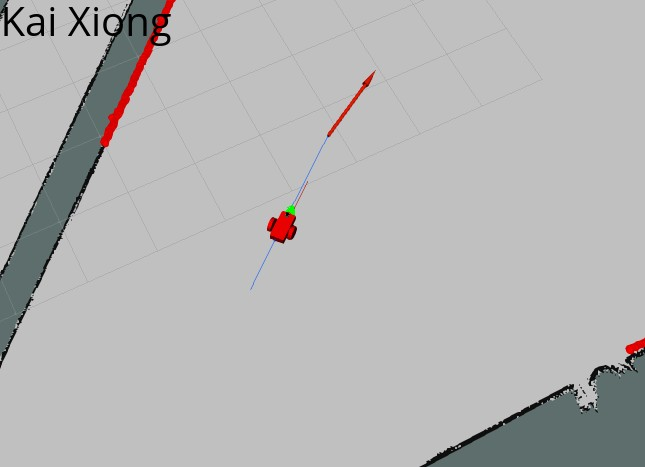
\includegraphics[width=\linewidth]{move_base.jpg}
      \caption{Localized Map.}
      \label{fig:robot4}
\end{figure}

\section{Discussion}
The AMCL performance depended on the CPU performance, laser scan accuracy and AMCL parameters. AMCL may perform badly in location such as long corridor, where there is less distinct feature in the map. MCL/AMCL can be used in application such as cleaning robot, service robot, transportation robot and AGV (Autonomous Guided Vehicle).

\section{Future work}
In conclusion, the custom mobile robot capable of accurately localized in a known map. Sensor fusion can help to improve the accuracy. Sensors such as IMU, RGBD camera and GPS. Robot\_pose\_ekf packages can perform sensor fusion by taking in sensors output. It can help to output more accurate position, even if one of the sensors is failed.

\end{document}